\documentclass{article}
\usepackage[utf8]{inputenc} %кодировка
\usepackage[T2A]{fontenc}
\usepackage[english,russian]{babel} %русификатор 
\usepackage{mathtools} %библиотека матеши
\usepackage[left=1cm,right=1cm,top=2cm,bottom=2cm,bindingoffset=0cm]{geometry} %изменение отступов на листе
\usepackage{amsmath}
\usepackage{graphicx} %библиотека для графики и картинок
\graphicspath{}
\DeclareGraphicsExtensions{.pdf,.png,.jpg}
\usepackage{subcaption}
\usepackage{pgfplots}

\begin{document}
% НАЧАЛО ТИТУЛЬНОГО ЛИСТА
\begin{center}
    \Large
    Федеральное государственное автономное \\
    образовательное учреждение высшего образования \\ 
    «Научно-образовательная корпорация ИТМО»\\
    \vspace{0.5cm}
    \large
    Факультет программной инженерии и компьютерной техники \\
    Направление подготовки 09.03.04 Программная инженерия \\
    \vspace{1cm}
    \Large
    \textbf{Отчёт по лабораторной работе №2} \\
    По дисциплине "Web программирование" \\
    \large
    \vspace{8cm}

    \begin{minipage}{.33\textwidth}
    \end{minipage}
    \hfill
    \begin{minipage}{.4\textwidth}
    
        \textbf{Студент}: \vspace{.1cm} \\
        \ Дениченко Александр P3212\\
        \textbf{Практик}:  \\
        \ Харитонова А. Е.
    \end{minipage}
    \vfill
Санкт-Петербург\\ 2023 г.
\end{center}

% КОНЕЦ ТИТУЛЬНОГО ЛИСТА 
\newpage

\section{Задание}
% 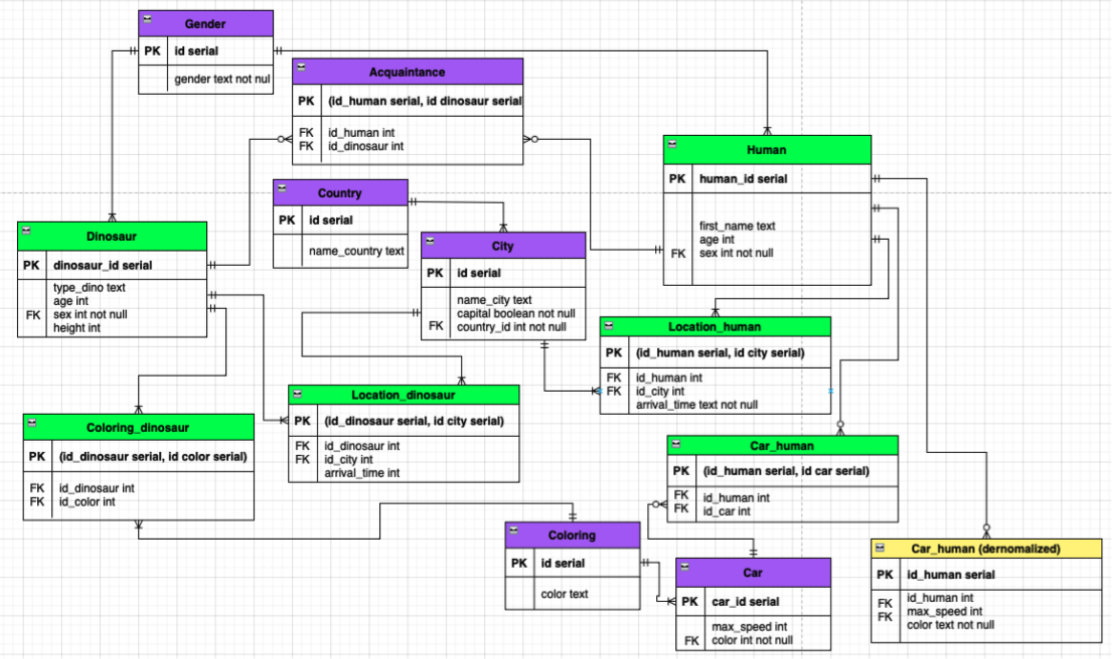
\includegraphics[width=.9\textwidth]{123}
Разработать веб-приложение на базе сервлетов и JSP, определяющее попадание точки на координатной плоскости в заданную область.

Приложение должно быть реализовано в соответствии с шаблоном MVC и состоять из следующих элементов:

ControllerServlet, определяющий тип запроса, и, в зависимости от того, содержит ли запрос информацию о координатах точки и радиусе, делегирующий его обработку одному из перечисленных ниже компонентов. Все запросы внутри приложения должны передаваться этому сервлету (по методу GET или POST в зависимости от варианта задания), остальные сервлеты с веб-страниц напрямую вызываться не должны.
AreaCheckServlet, осуществляющий проверку попадания точки в область на координатной плоскости и формирующий HTML-страницу с результатами проверки. Должен обрабатывать все запросы, содержащие сведения о координатах точки и радиусе области.
Страница JSP, формирующая HTML-страницу с веб-формой. Должна обрабатывать все запросы, не содержащие сведений о координатах точки и радиусе области.
Разработанная страница JSP должна содержать:

"Шапку", содержащую ФИО студента, номер группы и номер варианта.
Форму, отправляющую данные на сервер.
Набор полей для задания координат точки и радиуса области в соответствии с вариантом задания.
Сценарий на языке JavaScript, осуществляющий валидацию значений, вводимых пользователем в поля формы.
Интерактивный элемент, содержащий изображение области на координатной плоскости (в соответствии с вариантом задания) и реализующий следующую функциональность:
Если радиус области установлен, клик курсором мыши по изображению должен обрабатываться JavaScript-функцией, определяющей координаты точки, по которой кликнул пользователь и отправляющей полученные координаты на сервер для проверки факта попадания.
В противном случае, после клика по картинке должно выводиться сообщение о невозможности определения координат точки.
После проверки факта попадания точки в область изображение должно быть обновлено с учётом результатов этой проверки (т.е., на нём должна появиться новая точка).
Таблицу с результатами предыдущих проверок. Список результатов должен браться из контекста приложения, HTTP-сессии или Bean-компонента в зависимости от варианта.
Страница, возвращаемая AreaCheckServlet, должна содержать:

Таблицу, содержащую полученные параметры.
Результат вычислений - факт попадания или непопадания точки в область.
Ссылку на страницу с веб-формой для формирования нового запроса.
Разработанное веб-приложение необходимо развернуть на сервере WildFly. Сервер должен быть запущен в standalone-конфигурации, порты должны быть настроены в соответствии с выданным portbase, доступ к http listener'у должен быть открыт для всех IP.


\section{Код}
\begin{verbatim}
    package com.nordwestzap.weblab.dao;

    import com.nordwestzap.weblab.model.Attempt;
    import jakarta.ejb.Singleton;
    
    import java.io.Serializable;
    import java.util.ArrayList;
    import java.util.List;
    import java.util.Objects;
    import java.util.stream.Collectors;
    
    @Singleton
    public class AttemptRepository implements Serializable {
        private List<Attempt> attempts = new ArrayList<>();
    
        public AttemptRepository() {
        }
    
        public Attempt addAttempt(Attempt attempt) {
            attempts.add(attempt);
            return attempt;
        }
    
        public List<Attempt> getUserAttempts(String sessionId) {
            return attempts.stream()
                    .filter(attempt -> attempt.getSessionId().equals(sessionId))
                    .collect(Collectors.toList());
        }
    
        public void deleteUserAttempts(String sessionId) {
            attempts = attempts.stream()
                    .filter(attempt -> !attempt.getSessionId().equals(sessionId))
                    .collect(Collectors.toList());
        }
    
        public List<Attempt> getAttempts() {
            return attempts;
        }
    
        @Override
        public String toString() {
            return "AttemptRepository{" +
                    "attempts=" + attempts +
                    '}';
        }
    
        @Override
        public boolean equals(Object o) {
            if (this == o) return true;
            if (!(o instanceof AttemptRepository)) return false;
            AttemptRepository that = (AttemptRepository) o;
            return Objects.equals(attempts, that.attempts);
        }
    
        @Override
        public int hashCode() {
            return Objects.hash(attempts);
        }
    }
    package com.nordwestzap.weblab.model;

    public class Attempt {
    
        private final String sessionId;
        private final double x;
        private final double y;
        private final int r;
        private final boolean isHit;
        private final String attemptTime;
        private final long scriptDuration;
    
        public Attempt(String sessionId, double x, double y, int r, boolean isHit, String attemptTime, long scriptDuration) {
            this.sessionId = sessionId;
            this.x = x;
            this.y = y;
            this.r = r;
            this.isHit = isHit;
            this.attemptTime = attemptTime;
            this.scriptDuration = scriptDuration;
        }
    
        @Override
        public String toString() {
            return "Attempt{" +
                    "sessionId='" + sessionId + '\'' +
                    ", x=" + x +
                    ", y=" + y +
                    ", r=" + r +
                    ", isHit=" + isHit +
                    ", attemptTime='" + attemptTime + '\'' +
                    ", scriptDuration=" + scriptDuration +
                    '}';
        }
    
        public String getSessionId() {
            return sessionId;
        }
    
        public double getX() {
            return x;
        }
    
        public double getY() {
            return y;
        }
    
        public int getR() {
            return r;
        }
    
        public boolean isHit() {
            return isHit;
        }
    
        public String getAttemptTime() {
            return attemptTime;
        }
    
        public long getScriptDuration() {
            return scriptDuration;
        }
    }
    package com.nordwestzap.weblab.model;

    public class AttemptDto {
    
        private final double x;
        private final double y;
        private final int r;
        private final boolean isHit;
        private final String attemptTime;
        private final long scriptDuration;
    
        public AttemptDto(double x, double y, int r, boolean isHit, String attemptTime, long scriptDuration) {
            this.x = x;
            this.y = y;
            this.r = r;
            this.isHit = isHit;
            this.attemptTime = attemptTime;
            this.scriptDuration = scriptDuration;
        }
    
        public double getX() {
            return x;
        }
    
        public double getY() {
            return y;
        }
    
        public int getR() {
            return r;
        }
    
        public boolean isHit() {
            return isHit;
        }
    
        public String getAttemptTime() {
            return attemptTime;
        }
    
        public long getScriptDuration() {
            return scriptDuration;
        }
    }
    package com.nordwestzap.weblab.model;

    public class AttemptMapper {
    
        public static AttemptDto toAttemptDto(Attempt attempt) {
            return new AttemptDto(attempt.getX(), attempt.getY(), attempt.getR(), attempt.isHit(), attempt.getAttemptTime(), attempt.getScriptDuration());
        }
    }
    package com.nordwestzap.weblab;

    import com.fasterxml.jackson.databind.ObjectMapper;
    import com.nordwestzap.weblab.dao.AttemptRepository;
    import com.nordwestzap.weblab.model.Attempt;
    import com.nordwestzap.weblab.model.AttemptMapper;
    import jakarta.ejb.EJB;
    import jakarta.servlet.ServletException;
    import jakarta.servlet.http.Cookie;
    import jakarta.servlet.http.HttpServlet;
    import jakarta.servlet.http.HttpServletRequest;
    import jakarta.servlet.http.HttpServletResponse;
    
    import java.io.IOException;
    import java.time.Duration;
    import java.time.Instant;
    import java.time.LocalDateTime;
    import java.time.format.DateTimeFormatter;
    import java.util.List;
    import java.util.Objects;
    
    public class AreaCheckServlet extends HttpServlet {
    
        @EJB
        private AttemptRepository attemptRepository;
    
        @Override
        protected void doPost(HttpServletRequest request, HttpServletResponse response) throws ServletException, IOException {
    
            String xStr = (String) request.getParameter("x");
            String yStr = (String) request.getParameter("y");
            String rStr = (String) request.getParameter("r");
    
            if (xStr == null || yStr == null || rStr == null) {
                response.setStatus(400);
                response.getWriter().print("Request must contain x, y, r parameters");
                return;
            }
    
            double x = 0;
            double y = 0;
            int r = 0;
    
            try {
                x = Double.parseDouble(xStr);
            } catch (NumberFormatException e) {
                response.setStatus(400);
                response.getWriter().println("x must be integer value");
            }
    
            try {
                y = Double.parseDouble(yStr);
            } catch (NumberFormatException e) {
                response.setStatus(400);
                response.getWriter().println("y must be double value");
            }
    
            try {
                r = Integer.parseInt(rStr);
            } catch (NumberFormatException e) {
                response.setStatus(400);
                response.getWriter().print("r must be integer value");
            }
    
            if (response.getStatus() == 400)
                return;
    
            if (!(x>=-7 && x<=7)) {
                response.setStatus(400);
                response.getWriter().println("x must be integer value of [-4, -3, -2, -1, 0, 1, 2, 3, 4] ");
            }
    
            if (!(y >= -7 && y <= 7)) {
                response.setStatus(400);
                response.getWriter().println("y must be double value of (-3; 5)");
            }
    
            if (!(List.of(0, 1, 2, 3, 4, 5).contains(r))) {
                response.setStatus(400);
                response.getWriter().println("r must be integer value of [1, 2, 3, 4, 5]");
            }
    
            if (response.getStatus() == 400)
                return;
    
            Cookie sessionIdCookie = null;
            for (Cookie cookie : request.getCookies()) {
                if (cookie.getName().equals("JSESSIONID")) {
                    sessionIdCookie = cookie;
                    break;
                }
            }
            String sessionId = sessionIdCookie.getValue();
            String attemptTime = LocalDateTime.now().format(DateTimeFormatter.ofPattern("u-M-d k-m-s"));
            Instant start = Instant.now();
            boolean isHit = checkHit(x, y, r);
            Instant end = Instant.now();
            long scriptDuration = Duration.between(start, end).toNanos();
    
            Attempt attempt = attemptRepository.addAttempt(new Attempt(sessionId, x, y, r, isHit, attemptTime, scriptDuration));
    
            ObjectMapper objectMapper = new ObjectMapper();
            response.setStatus(200);
            response.getWriter().print(objectMapper.writeValueAsString(AttemptMapper.toAttemptDto(attempt)));
    
        }
    
        private boolean checkHit(double x, double y, int r) {
            if ((x >= 0 && x <= r) && (y >= 0 && y <= r))
                return Math.pow(x, 2) + Math.pow(y, 2) <= Math.pow(r, 2);
            else if ((x <= 0 && x >= -r) && (y >= 0 && y <= (double) r / 2))
                return y <= (double) r / 2;
            else if (x < 0 && y < 0)
                return false;
            else if ((x >= 0 && x <= r) && (y <= 0 && y >= -r))
                return y >= x - r;
            else
                return false;
        }
    
    }
    package com.nordwestzap.weblab;

    import com.nordwestzap.weblab.dao.AttemptRepository;
    import jakarta.ejb.EJB;
    import jakarta.servlet.ServletException;
    import jakarta.servlet.http.Cookie;
    import jakarta.servlet.http.HttpServlet;
    import jakarta.servlet.http.HttpServletRequest;
    import jakarta.servlet.http.HttpServletResponse;
    
    import java.io.IOException;
    
    public class ControllerServlet extends HttpServlet {
    
        @EJB
        private AttemptRepository attemptRepository;
    
        @Override
        protected void doGet(HttpServletRequest request, HttpServletResponse response) throws ServletException, IOException {
    //        System.out.println("get req");
            request.setAttribute("Attempt-Repository", attemptRepository);
            request.getRequestDispatcher("/index.jsp").forward(request, response);
        }
    
        @Override
        protected void doPost(HttpServletRequest request, HttpServletResponse response) throws ServletException, IOException {
    //        System.out.println("post req");
            request.getRequestDispatcher("/check").forward(request, response);
        }
    
        @Override
        protected void doDelete(HttpServletRequest request, HttpServletResponse response)
                throws ServletException, IOException {
    
            Cookie sessionIdCookie = null;
            for (Cookie cookie : request.getCookies()) {
                if (cookie.getName().equals("JSESSIONID")) {
                    sessionIdCookie = cookie;
                    break;
                }
            }
    
            //TODO check cookie
            String sessionId = sessionIdCookie.getValue();
    
            attemptRepository.deleteUserAttempts(sessionId);
    
            response.setStatus(HttpServletResponse.SC_OK);
    //        response.getWriter().write("Запрос DELETE успешно обработан.");
        }
    }
    package com.nordwestzap.weblab;

    import jakarta.servlet.FilterChain;
    import jakarta.servlet.ServletException;
    import jakarta.servlet.http.HttpFilter;
    import jakarta.servlet.http.HttpServletRequest;
    import jakarta.servlet.http.HttpServletResponse;
    
    import java.io.IOException;
    
    public class UrlFilter extends HttpFilter {
    
        @Override
        protected void doFilter(HttpServletRequest request, HttpServletResponse response, FilterChain chain) throws IOException, ServletException {
            String uri = request.getRequestURI();
            if (uri.endsWith("/lab") || uri.endsWith("/index.js")) {
                request.getServletContext().getNamedDispatcher("ControllerServlet").forward(request, response);
            } else if(uri.endsWith("/")){
                response.sendRedirect(uri+"lab");
            }
            else  {
    //            System.out.println("доступ ограничен "+request.getRequestURI());
                response.setStatus(404);
            }
        }
    
    }
                   
\end{verbatim}
\section{Вывод}
Разработали сайт, используя сервлеты их контейнер, jsp. Для контейнера сервлетов был выбран Wild-fly. Сайт запущен на удалённом сервере helios, проброщены порты.
\end{document}

